\documentclass[12pt,subf,href,colorlinks=true]{article}



\usepackage[a4paper,nohead,includefoot,mag=1000,
            margin=2cm,footskip=1cm]{geometry}
%\usepackage[T2A]{fontenc}
%\usepackage[cp1251]{inputenc}
%\usepackage{pscyr}
%\renewcommand{\rmdefault}{ftm}
\usepackage{cmap}
\usepackage[utf8]{inputenc}
%\usepackage[TS1,T2A]{fontenc}
\usepackage[russian]{babel}
\usepackage{tabularx}
\usepackage{hyperref}
\ifpdf\usepackage{epstopdf}\fi
\hypersetup{
    colorlinks=true,
    linkcolor=blue,
    filecolor=magenta,      
    urlcolor=blue,
}
\usepackage{listings}
\usepackage{algorithm}
\usepackage{algpseudocode}
\usepackage{placeins}


\title{Задание №3: Программная реализация графического конвейера и графического API}
\author{Владимир Фролов}
\date{\today}

\usepackage{graphicx}
\graphicspath{{img/}}
\renewcommand{\baselinestretch}{1.25}

% listings

\usepackage{color} 
\usepackage{listings} 
\usepackage{caption}
\DeclareCaptionFont{white}{\color{white}} 
\DeclareCaptionFormat{listing}{\colorbox{gray}{\parbox{\textwidth}{#1#2#3}}}
\captionsetup[lstlisting]{format=listing,labelfont=white,textfont=white}


\lstset{ %
language=C,                
stepnumber=1,              
tabsize=2,                 
}

\begin{document}
\maketitle

\begin{abstract}
	
\noindent Цель задания: закрепить на практике основные работы графического конвейера через его реализацию.

\begin{itemize}

\item Закрепление знаний о трёхмерных преобразованиях и базовых математических операциях.
\item Изучение базовых принципов работы графического конвейера;
\item (Дополнительно) Программируемая функциональность граф-конвейера.
\item (Дополнительно) Карты теней	 
	 
\end{itemize}	

\end{abstract}


\begin{figure}
	\begin{center}
		\begin{tabular}{c c}
			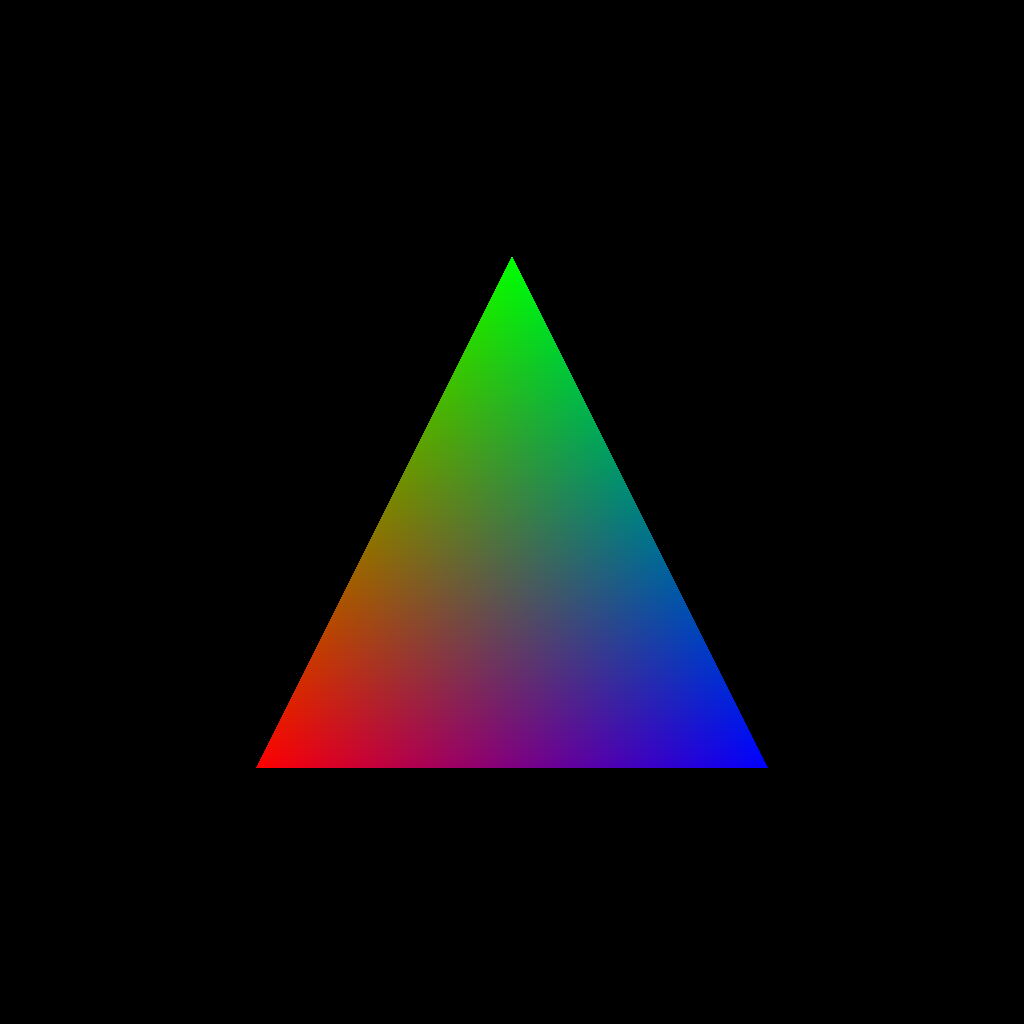
\includegraphics[width=0.25\textwidth]{img/wref_01.png} & 
			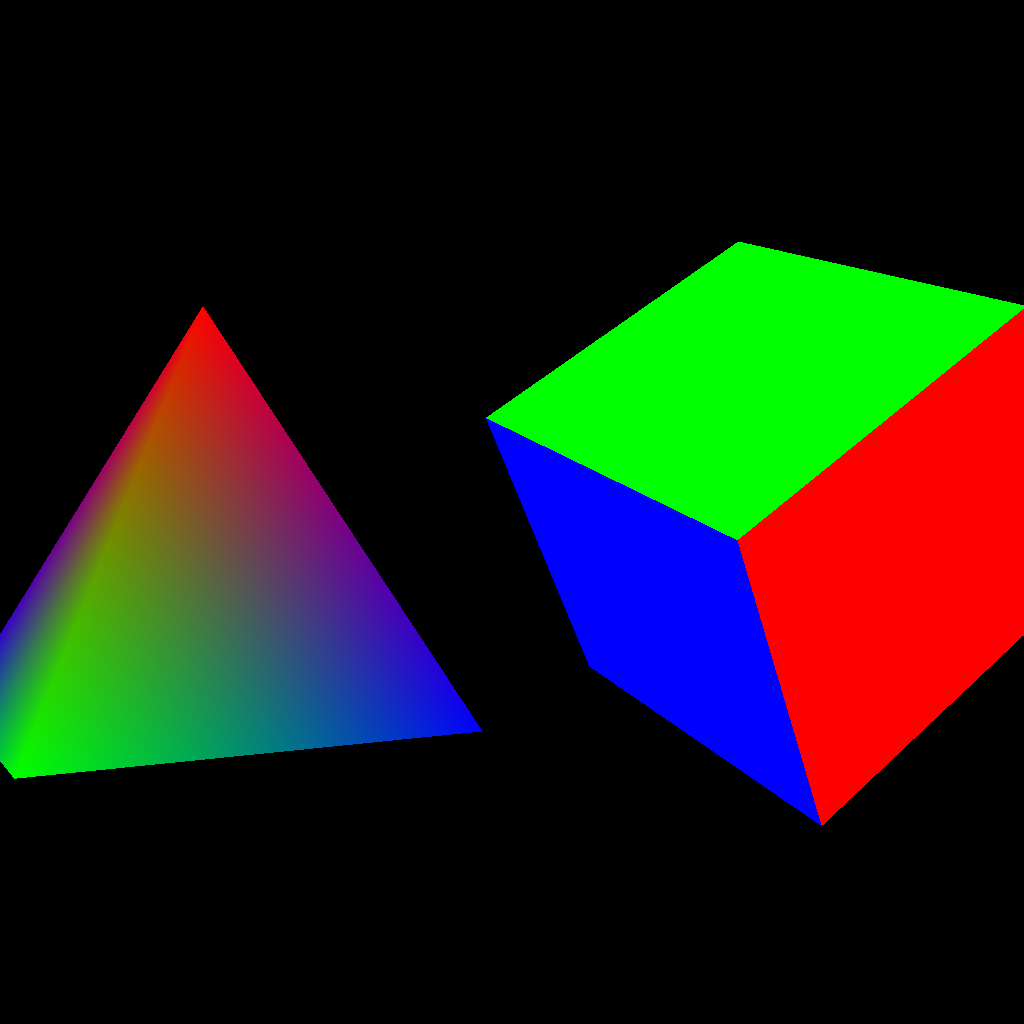
\includegraphics[width=0.25\textwidth]{img/wref_03.png} \\ 
			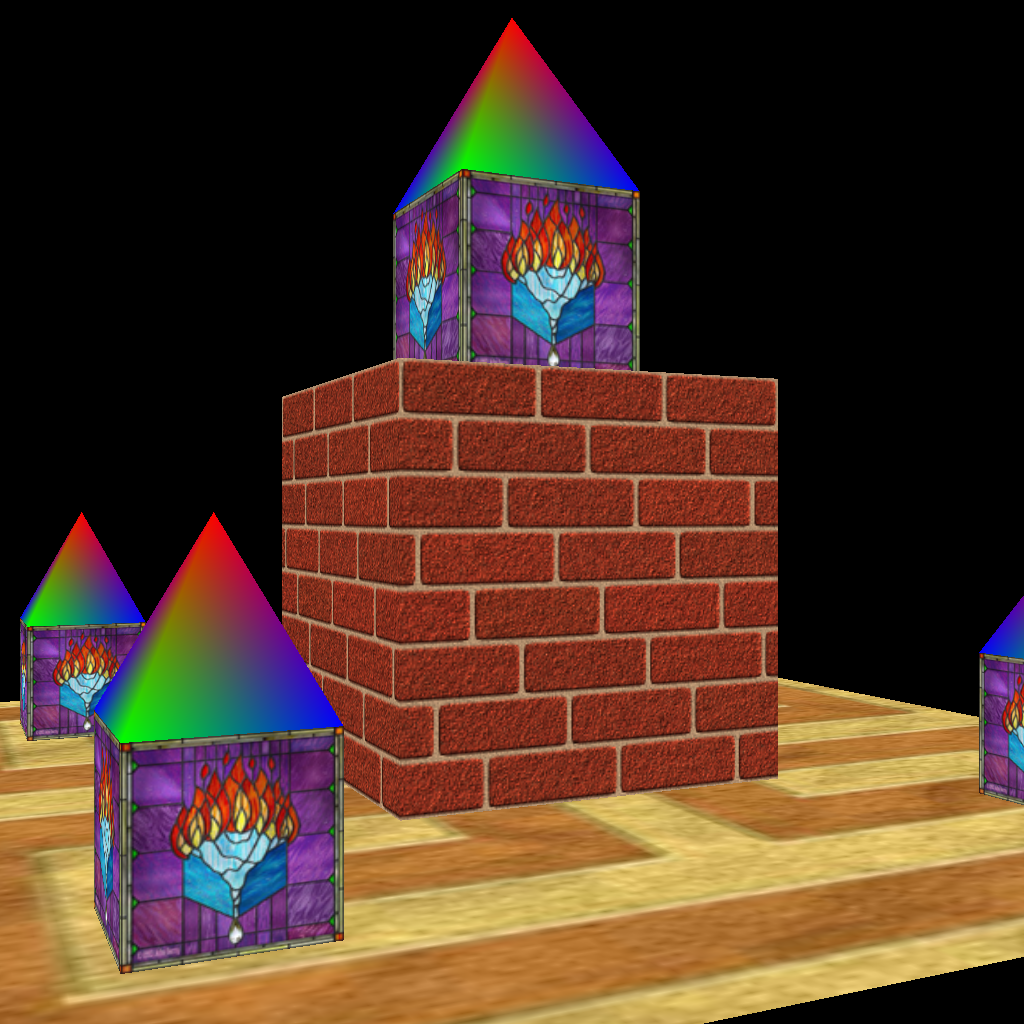
\includegraphics[width=0.25\textwidth]{img/wref_05.png} &
			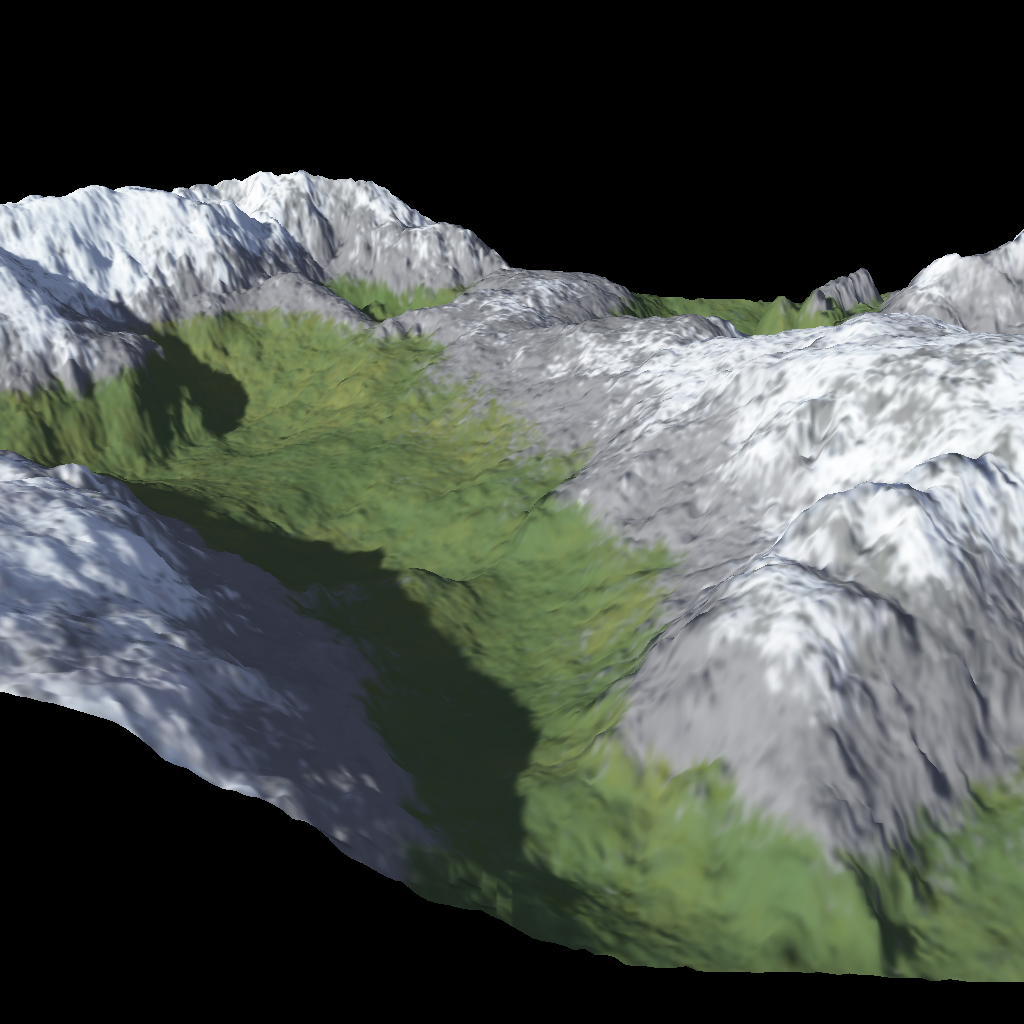
\includegraphics[width=0.25\textwidth]{img/wref_08.png} \\
		\end{tabular}
		\caption{Изображения некоторых тестовых сцен}
		\label{fig:images}
	\end{center}
\end{figure}

\section{Базовая часть: 10 баллов }

Необходимо реализовать базовый алгоритм растеризации 3D моделей с поддержкой текстурирования.

\begin{itemize}
  \item Необходимо реализовать заливку треугольника константным цветом (1 балл).
  \item Необходимо реализовать интерполяцию цвета (2 балла).
  \item Необходимо реализовать интерполяцию текстурных координат с перспективной коррекцией (3 балла).
  \item Необходимо реализовать алгоритм буфера глубины для корректного отображения ближних и дальних объектов (4 балла).
  \item Для каждого изображения необходимо вывести время его рендеринга. При невыполнении этого требования баллы за базовую часть будут снижены вдвое!
  \item К заданию прилагается эталонная реализация через OpenGL 1.0. Для успешного выполнения задания необходимо получить хотя бы похожие (а в идеале совпадающие) с эталонными изображения на всех 8 тестах (рис. \ref{fig:images}). При невыполнении этого требования баллы за базовую часть будут снижены на усмотрение проверяющего.
\end{itemize}

\section{Дополнительная часть: 15 баллов макс.}

\begin{itemize}
	
	\item Синтез последовательности изображений, содержаших поворот сцены вокруг центра координат или вращение некоторой 3D модели вокруг её центра (+1 балл). 
  
    \begin{itemize}
    \item Используйте ffmpeg чтобы получить видео-последовательность из набора изображений:
    \begin{verbatim}ffmpeg -framerate 25 -pattern\_type glob -i '*.bmp' out.gif \end{verbatim}
    
    \item В качестве альтернативного решения Вы можете выводить изображений в окно (проверка вашего задания будет осущесвлятьтся на Linux с оконной системой X11, как в примере для эталонной реализации). В этом случае пожалуйста выведите частоту кадров в название окна или в командную строку.
    \end{itemize}
    
    \item Реализация прозрачности при помощи альфа-смешивания (2 балла для выпуклых объектов и 3 балла для не-выпуклых).
    
    \begin{itemize}
    	\item Добавьте новый режим и (при необходимости) новые поля в структуру \newline PipelineStateObject
    	
    	\item Добавьте режим отбраковки задних или передних поверхностей (по порядку обхода вершин -- по часовой стрелки или против). Этот необходимо сделать т.к. для корректного отображения прозрачных объектов Вам сначала придётся рисовать задние грани, а затем передние
    	
    	\item Для не-выпуклых объектов необходимо реализовывать сортировку граней по расстоянию от камеры (координата z в пространстве камеры после применения worldView матрицы). 
    \end{itemize}
    
	\item Загрузка и рендеринг ``.obj'' файлов (3 балла).
    \begin{itemize}
    	\item Необходимо реализовать визуализацию как минимум 2 разных моделей
    	\item Вы можете использовать и другой входной формат 3D моделей.
    \end{itemize}		
		
	\item Реализия фрагментных шейдеров через указатели на функции (или аналогичную функциональность вашего языка программирования) (3 балла).
	
	\begin{itemize}
	  \item Добавьте необходимую входную информацию в структуру PipelineStateObject;	
	  \item Необходимо реализовать рассчёт освещения во фрагментном шейдере (без этого пункт не засчитывается).
	\end{itemize}

    \item Блочный алгоритм растеризации (2 балла).
    
    \item Применение векторизацию кода для блочного растеризатора и фрагментных шейдеров при помощи Intel ISPC (2 балла).
    
    \begin{itemize}
      \item В этом пункте необходимо реализовать рассчёт освещения во фрагментном шейдере (без этого пункт не засчитывается).
      \item Все векторизованные шейдеры должны быть собраны в объектные файлы и статически прилинкованы к проекты.
      \item Необходимо привести сравнение времени выполнения для обычных и векторизованных шейдеров.
    \end{itemize}
	
	\item Необходимо реализовать алгоритм карт теней. Необходимо продемонстрировать самозатенение или отбрасывание теней с одного 3D объекта на другие (4 балла).
	
	\item Растеризация квад-мешей  (+3 балла).
	\begin{itemize}
	  \item В последнее время стали популярны меши, состоящие из четырё-угольников \cite{quadmeshes_about}. Преобразование таких мешей в треугольные снижает эффективность блочных алгоритмов растеризации на границе двух треугнольников, образующих квад. Необходимо реализовать алгоритм растеризации квадов и сравнить время работы с растеризацией треугольников.
	  
	  \item Существенно-непланарные квады необходимо всё-равно разбивать на треугольники.
	  
	  \item Данный пункт имеет смысл выполнять только если Вы реализуете блочный векторизованный алгоритм. 
	  
	  \item Подготовленные для задания квад-меши можно найти здесь: \cite{quadmeshes}. 
	   
	\end{itemize}
	
\end{itemize}

\section{Порядок выполнения задания}

\begin{enumerate}
\item Скачайте или склонируйте себе шаблон для выполнения задания \cite{ourtemplate}
  \begin{itemize}
	\item Пожалуйста не выкладывайте Ваше \textbf{решение} в открытый доступ. Дайте возможность другим людям достичь результата самостоятельно.
  \end{itemize}

\item Соберите шаблон с эталонной реализацией и сгенерируйте эталонные изображения
  \begin{itemize}
  \item \begin{verbatim} mkdir build && cd build \end{verbatim}
  \item \begin{verbatim} cmake -DCMAKE_BUILD_TYPE=Release (или Debug) -DUSE_OPENGL=ON .. \end{verbatim}
  \item \begin{verbatim} make -j 8 \end{verbatim}
  \item Запустите полученную програму
  \end{itemize}

\item Отключите эталонную реализацию и приступайте к выполнению задания
   \begin{itemize}
  	\item \begin{verbatim} cmake -DCMAKE_BUILD_TYPE=Release (или Debug) -DUSE_OPENGL=OFF .. \end{verbatim}
  	\item \begin{verbatim} make -j 8 \end{verbatim}
  \end{itemize}

\item Эталонная реализация создаёт окно при помощи X11, поэтому если в Вашей системе это невозможно, попросите товарища сгенерировать эталонные изображения для Вас.

\item Если Вы хотите выполнить задание на другом языке программирования, это допускается при условии совпадения вашей реализации с эталонными изображениями. 

\item Изучите раздел \ref{materials} (Материалы для выполнения задания) и сайт \cite{scratchpixel}.

\end{enumerate}

\section{Порядок сдачи}
Ваша программа должна запускаться без аргументов, производить рендеринг изображений и сохранить их на выходе в bmp формат. Если Вы создаёте окно, то примите во внимание что проверка будет производитьcя на машинах Linux и оконной системой X11 (XWindow).
 
\noindent\textbf{Использование библиотек}: 

Все используемые библиотеки должны быть либо собраны в статические библиотеки для архитектуры x64 c поддержкой AVX2 (-mavx2) под gcc, либо должны поставляться с проектом в виде исходных кодов, и фактически быть его частью. PS: строго говоря, для выполнения данного задания Вам не нужны библиотеки. Рекомендуется выполнять задание без них. 

\section{Именование архива}

Архив, который вы загружаете на сайт должен называться по следующему шаблону: \newline <номер\_группы>\_<фамилия>.zip. Фамилию следует писать латинскими символами.

\section{Материалы для выполнения задания}\label{materials}

Итак, Вам выдали это скучнейшее в мире задание c растеризацией треугольников, в котором зачем-то требуется совпадение Вашей реализации с эталонной, написанной на умершем уже 10 лет как OpenGL 1.0. Что-ж, на практике Вам действительно придётся использовать другие API, шейдеры, GPU и многое другое. Поэтому совершенно точно можно сказать, что выполнив это задание Вы не получите практических навыков. Зато Вы получите громадный буст к их освоению, поскольку будете понимать как графические API, граф. конвейер (и даже современные GPU) устроены изнутри. Ведь в действительности там всё не так сложно, как кажется на первый взгляд.

\subsection{Вопрос дизайна графического API}

Современные графические API прошли достаточно длинный и не всегда эволюционный (а скорее наоборот) путь развития. Поэтому вопрос их дизайна не такой простой как может показаться на первый взгляд. Вам предлагается реализовать учебный GAPI, в котором функциональность урезана до минимума. Если он Вам не нравится, Вы можете придумать свой API и реализовать предложенный через него или переделать предложенные примеры на свой вариант интерфейса. Опишем требования, которые определяют дизайн нашего учебного API и обсудим особенности дизайна:

\begin{enumerate}
\item В базовой части задания необходимо отрисовывать непосредственно цвет в формате RGB, причём в двух режимах.
\begin{enumerate}
\item Цвет задаётся в вершинах 3D модели
\item Цвет задаётся текстурой, а в вершинах 3D модели заданы текстурные координаты
\item В дополнительной части задания Вы можете расширить API для задания программируемой функциональностью, прозрачностью и др.
\end{enumerate}

\item Режим отрисовки задаётся структурой PipelineStateObject. Такая структура так или иначе есть во всех графических API. Она полностью определяет то, как именно производится отрисовка определённой 3D модели и может содержать внутри себя ссылки на другие структуры (юниформы, шейдеры, состояния растеризатора и т.п.). Обратите внимание, что помимо режима отриcовки и идентификатора текстуры мы добавили в неё две матрицы -- worldViewMatrix и projMatrix. Можно было бы отделить матрицы в отдельную структуру (назовём её Uniforms), но на самом деле это не влияет на суть дела, поскольку в конечном итоге для правильной отрисовки необходимо иметь всю информацию о состоянии граф. конвейера, в том числе и юниформы.

\item Структура Geom задаёт саму 3D модель. Вам не нужно поддерживать различные способы (лэйауты, форматы) хранения геометрии. В данном задании геометрия хранится в одном, строго фиксированном представлении.

\item Инстансинг. Обычно для того чтобы отрисовать одну 3D модель несколько раз с разными 3D преобразованиями в GAPI добавляют специальные функции (вроде glDrawElementsIndexedInstanced). В нашем случае мы делаем это более явно, изменяя PipelineStateObject для кажого вызова Draw (с.м. функцию DrawInstances). То есть явной поддержки инстансинга в нашем GAPI нет. Тем не менее исходно геометрия организована таким образом, чтобы её можно было отрисовывать с инстансингом, поэтому при желании Вы можете добавить поддержку этой функциональности в API (баллов за это не даётся). 

\item Изображения. Нетрудно заметить, что изображение в предлагаемом API является легковесным объектом, а сами данные при этом расположены где-то ещё (как, например, это сделано в Vulkan). AddImage предполагает что Вы будете копировать входное содержимое изображения куда-то внутрь вашего API. Однако Вы можете изменить код в main.cpp так чтобы все загруженные изображения находились в различных векторах, вектора эти не удалялись и, таким образом, вам не нужно будет копировать данные изображений, а достаточно только скопировать ссылки на них, то есть саму структуру Image2D. Каковы последствия такого изменения?  

\begin{enumerate}
	\item Преимущество в том, что ваш API, по сути, вообще не будет выделять внутри себя память (кроме Z-буфера, но и это можно исправить при желании). Это существенно для приложений повышенной надёжности и различных встраиваемых систем, где аллокация памяти строго статическая. Обратите внимание, что похожая концепция строгого контроля и не-выделения лишней памяти присутствует в Vulkan.
	 
	\item Недостаток такого решения в том, что Вы не можете просто так втихую применить какие-то оптимизации. Например, хранить текстуру блоками, уменьшить битность текстуры или сделать обработку границ через добавление т.н. ``юбки'' вокруг текстуры (последнее является существенной оптимизацией в программных решениях при реализации текстурной выборки). А при копировании данных внутрь Вы можете это сделать.
	
	\item Именно по причине необходимости применения различных оптимизаций в Vulkan, например, мы имеем такой непростой порядок действий. Сначала Вы запрашиваете у API сколько памяти нужно для такой-то текстуры, потом выделяете память, и лишь затем создаёте объект текстуры который привязываете к выделенной памяти.
\end{enumerate}

\item Рендер-пасс. Это понятие призвано сгруппировать определённую последовательность действий и/или функций отрисовки \textbf{в определённое изображение}.

\begin{enumerate}
	\item В простейшей реализации Вы очищаете нулями изображение в начале работы (\textit{BeginRenderPass}) и сихронизируете работу вашего апи в конце (\textit{EndRenderPass}) если, например, Вы используете многопоточность.
	
	\item Более сложный вариант может предполагать, что у Вас есть внутреннее представление буфера кадра, которой может храниться, например, тайлами 4x4. Такой формат повышает производительность блочных алгоритмов растеризации. В этом случае в \textit{EndRenderPass} Вы также должны скопировать ваш внутренний буфер кадра в выходное изображение. Обратите внимание, что именно с подобными оптимизациями связаны связаны лэйауты текстур в Vulkan и тот факт, что рендер-пасс умеет их менять.
	
	\item Убедитесь что пользователь передаёт одно и то же изображение как в \textit{BeginRenderPass}, так и в \textit{EndRenderPass}. Гипотетически, нетрудно развить API таким образом, чтобы подержать одновременную отрисовку в различные изображения.
\end{enumerate}


\end{enumerate}

\subsection{Стадии графического конвейера}

Современный графический конвейер может быть представлен как набор параллельных процессов, где различные стадии конвейера связаны друг с другом по схеме производитель-потребитель (рис. \ref{fig:prodcons}). При этом предполагается, что данные передающиеся между стадиями, не выгружаются в оперативную память из сверх-оперативной, а передаются между потоками/выч.устройствами каким-то более эффективным способом. 

\begin{figure}[h]
	\centering{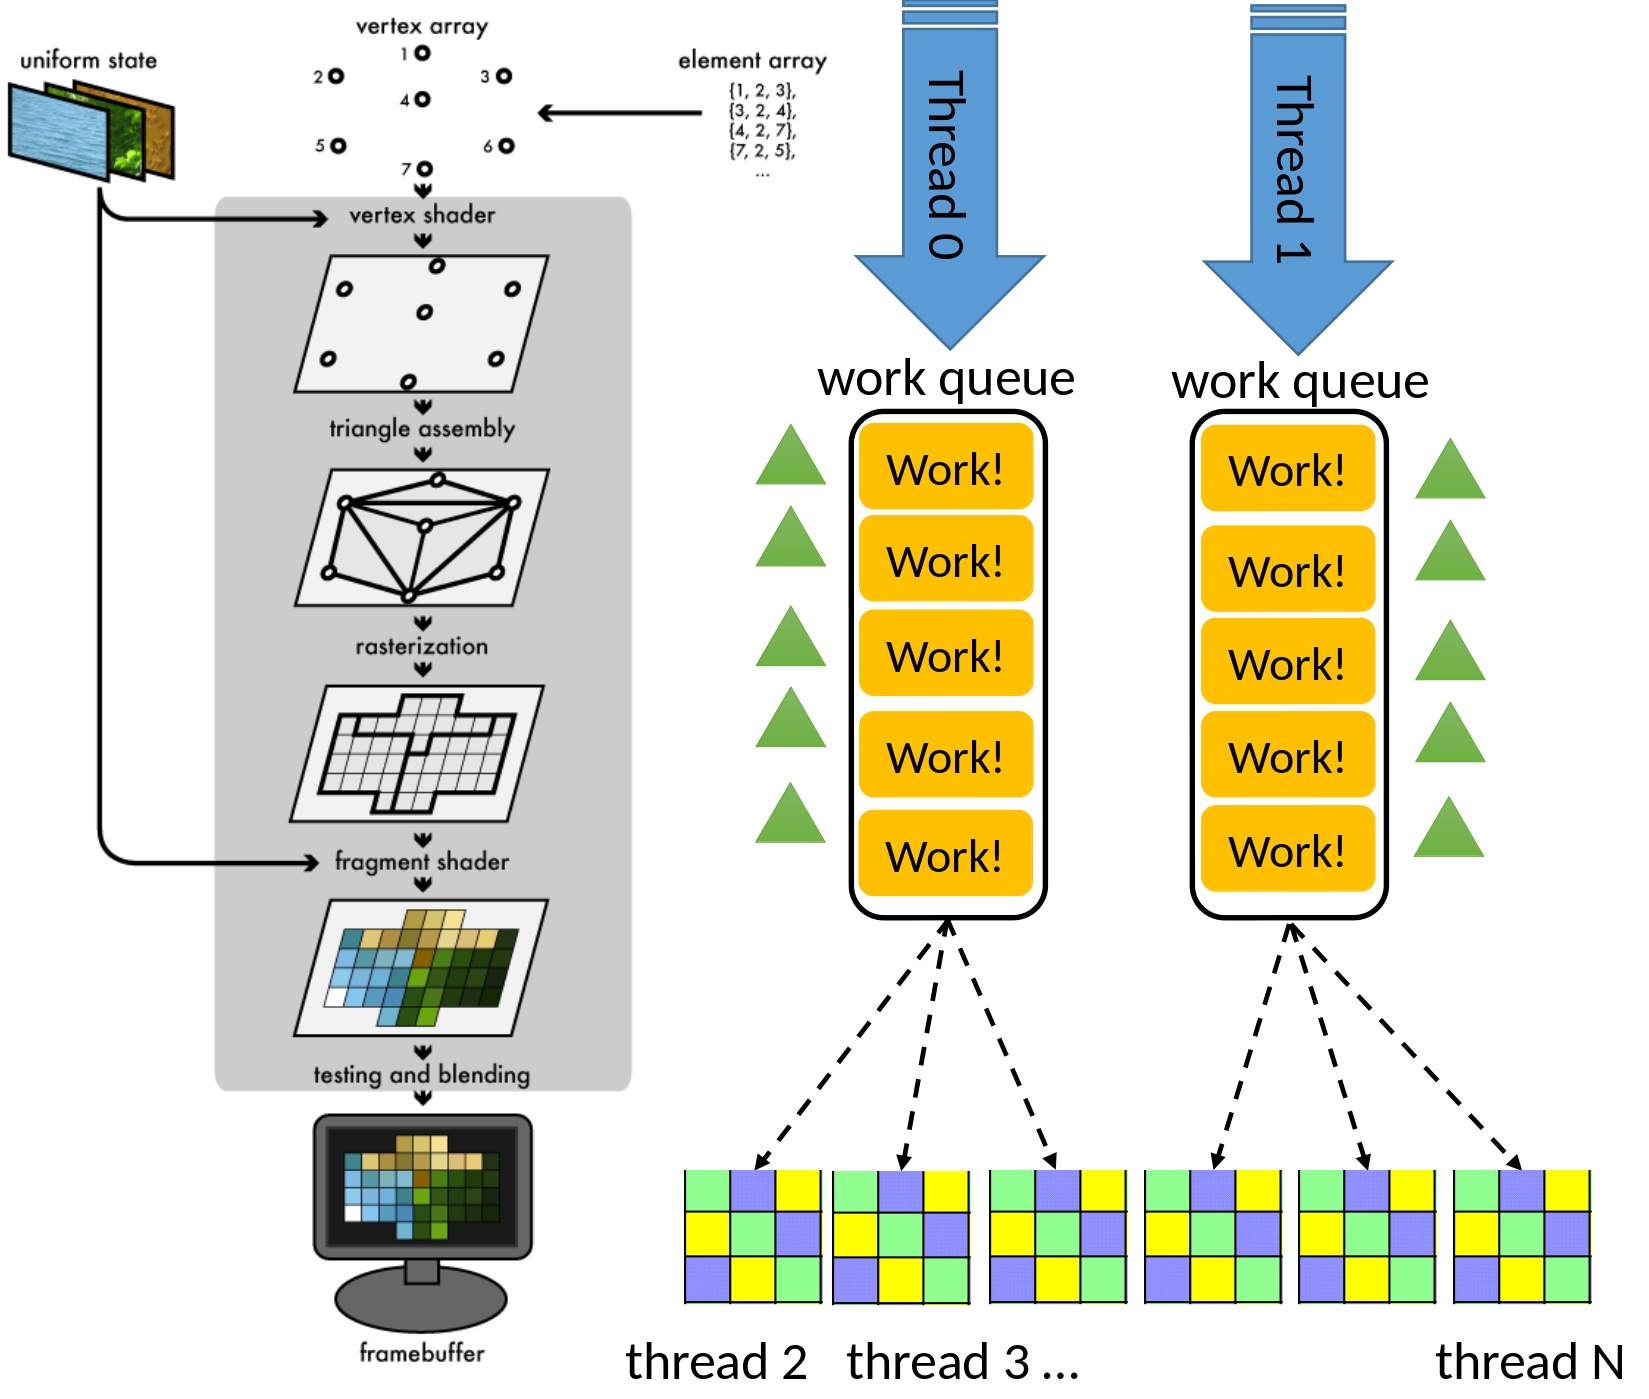
\includegraphics[width=0.5\linewidth]{img/graphicspipeline}}
	\caption{Графический конвейер устроен по схеме производитель-потребитель, где каждая стадия принимает на вход порцию данных, обрабатывает её и передаёт ниже по конвейеру. Как правило, обработка фрагментов гораздо тяжелее геометрических стадий. }
	\label{fig:prodcons}
\end{figure}

Эффективная реализация такой схемы на современных вычислительных системах является нетривиальной задачей, поэтому многие программные решения просто распараллеливание отдельные стадии конвейера. Именно по этой причине в вашем задании параллельной реализации не требуется, и баллов за неё не даётся. Хотя Вы можете это сделать.

Итак, Вам необходимо реализовать следующую последовательность действий.

\begin{enumerate}
\item Вершинный шейдер;
\begin{enumerate}
  \item До выполнения вершинного шейдера необходимо перемножить матрицы proj и worldView, чтобы получить единственную матрицу, которая осуществляет преобразование из мирового пространства в т.н. NDC пространство (Normalized Device Coordinates -- единичный куб от -1 до 1).
  \begin{verbatim} worldViewProj = projMatrix*worldView; \end{verbatim}
  
  \item Необходимо умножить полученную матрицу worldViewProj на все вершины и, таким образом, преобразовать их.
  
  \item Полученный вектор необходимо поделить на четвёртую координату ``w'' для того чтобы перейти от \textbf{Однородных Координат} \cite{ignatenkocoords} к декартовым. 
  
  \begin{verbatim} vNDC[i] = worldViewProj*vpos4f[i];  \end{verbatim}
  \begin{verbatim} vNDC[i] /= vNDC[i].w; \end{verbatim}
  
  \item Итоговый вектор vNDC[i] необходимо перевести в пространство экрана:
  \begin{verbatim} x = vNDC[i].x*0.5 + 0.5   // [-1,1] -> [0,1]  \end{verbatim}
  \begin{verbatim} y = vNDC[i].y*0.5 + 0.5   // [-1,1] -> [0,1]  \end{verbatim}
  \begin{verbatim} x_screen = x*width  - 0.5 // [0,1] -> [0,width] \end{verbatim}
  \begin{verbatim} y_screen = y*height - 0.5 // [0,1] -> [0,height] \end{verbatim}
  
  \item В предлагаемом API матрицы хранятся по строчкам в целях упрощения их восприятия. Однако внутри вашей реализации мы рекомендуем хранить матрицы по столбцам. Это позволяет компилятору оптимизировать умножение матрицы на точку с использованием векторных команд (используйте сайт godbolt \cite{godbolt} для проверки!).
  
\end{enumerate}	
\item Подготовка данных треугольников (TriangleSetUp или сборка примитивов). Эта стадия довольно проста. Её смысл заключается в том чтобы собрать все данные необходимые для растеризации треугольника в одну структуру, которая дальше передаётся по конвейеру. Поэтому всё что Вы должны сделать -- прочитать три вершины треугольника по трём индексам из массива преобразованных вершин. 

\begin{enumerate}
\item Вы могли бы объединить стадию вершинного шейдера и стадию подготовки треугольника, однако в этом случае для вершин, входящих более чем в один треугольник вершинный шейдер выполнится более одного раза.

\item Именно с этой проблемой связан т.н. T\&L cache \cite{TnLCache}, суть которого в том, чтобы закэшировать некоторое количество преобразованных вершин чтобы далее сразу же передать их на стадию TriangleSetUp из вершинного шейдера, не выгружая в оперативную память. 
\end{enumerate}	

\item Если Вы реализуете отбраковку обратных поверхностей по их порядку обхода, то именно на этой стадии.

\item Растеризация треугольников. Мы предлагаем Вам реализовать алгоритм растеризации на основе полу-пространства (в базе) и его блочную версию в дополнительной части. Подробности см. в следуюшем разделе.

\item В целях упрощения задания мы намеренно опускаем вопрос отсечения треугольников по ближней плоскости отсечения. В тестовых сценах геометрия расположена таким образом, что отсечение делать не требуется. Вам нужно лишь убедиться, что ограничивающий примитив прямоугольник не выходит за границу экрана.  
\end{enumerate}


\subsection{Алгоритм растеризации на основе полу-пространства}

Идея алгоритма растеризации на основе полу-пространства довольно проста: вы сканируете все пиксели в ограничивающем Ваш примитив прямоугольнике и проверяете, лежат центры пикселей внутри треугольника или снаружи (рис \ref{fig:halfspace_and_coverage} b). В первом задании Вы уже сталкивались с функциями расстояния и решали подобную задачу для произвольных фигур. Так называемая edge-функция это и есть знаковое расстояние до ребра треугольника (формула \ref{eq:edgefunction}).

\begin{equation}\label{eq:edgefunction}
	E(A,B,P) = (P.x - A.x) (B.y - A.y) - (P.y - A.y)(B.x - A.x)
\end{equation}

Здесь $A$ и $B$ две вершины ребра, а точка $P$ -- произвольная точка на плоскости изображения. Далее Вы просто реализуете вычисление этой функции для всех трёх рёбер треугольника $E_{\alpha}(x,y)$, $E_{\beta}(x,y)$, $E_{\gamma}(x,y)$: (формулы \ref{eq:edgefunction1}--\ref{eq:edgefunction3}, рис \ref{fig:halfspace_and_coverage} a)

\begin{figure}
	\begin{center}
		\begin{tabular}{c c}
			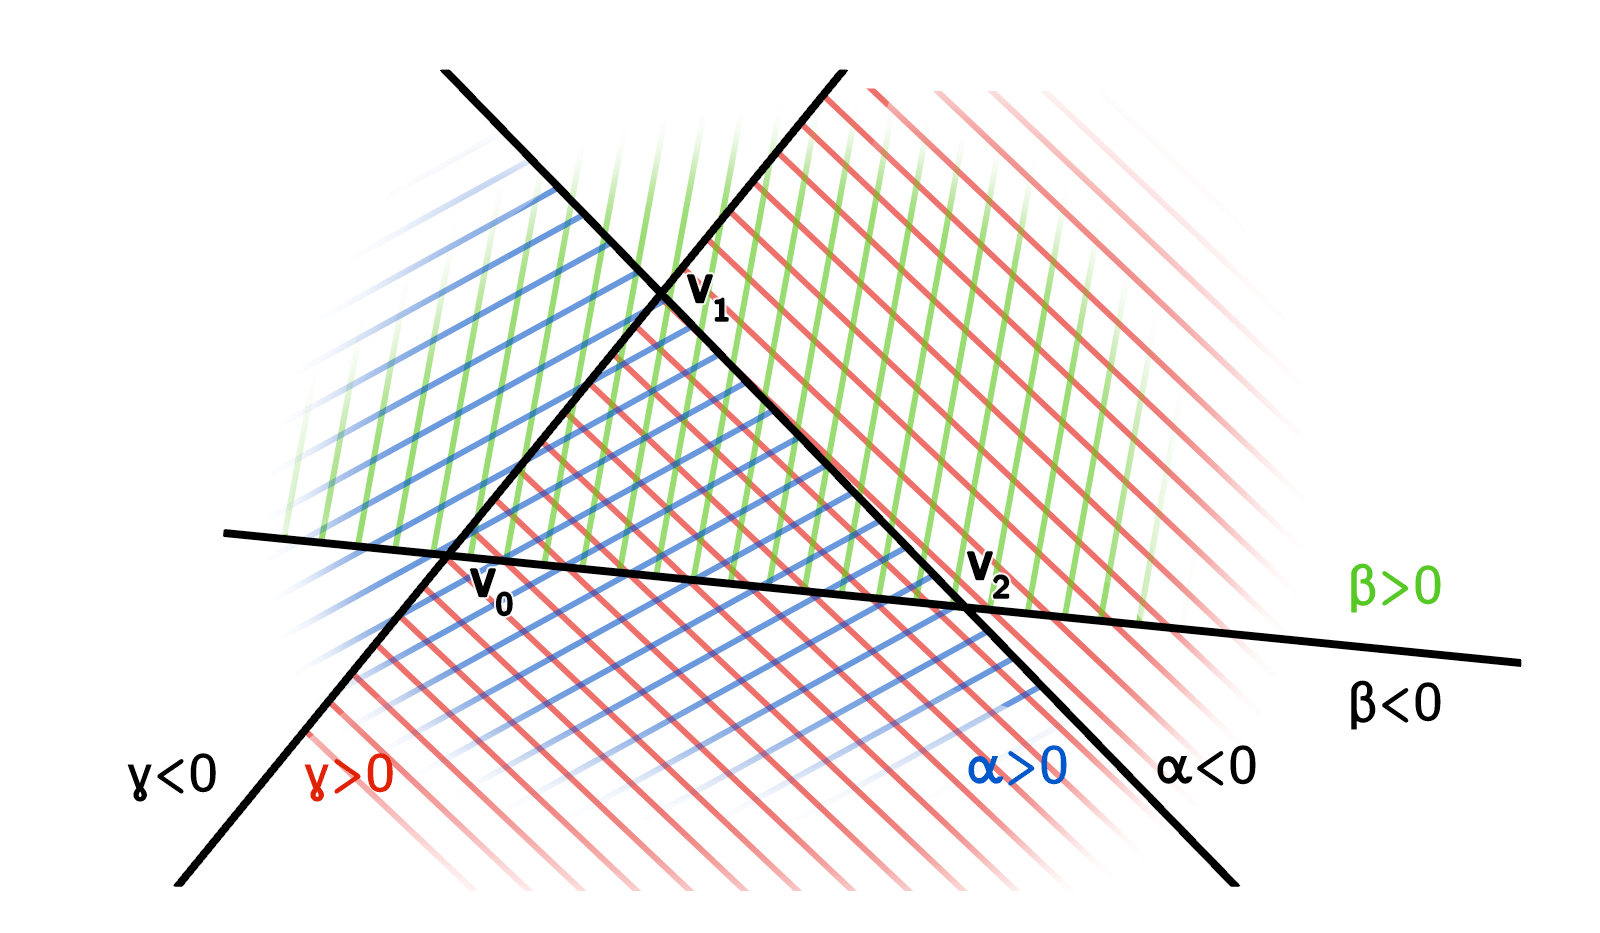
\includegraphics[width=0.5\textwidth]{img/barycentric} & 
			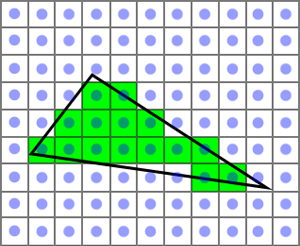
\includegraphics[width=0.325\textwidth]{img/coveragetest} \\
			 (a) & (b)
		\end{tabular}
		\caption{Принцип работы растеризатора на основе полу-пространства (a); Стандартное поведение теста на перекрытие пиксела треугольником проверяет центр пиксела (b).}
		\label{fig:halfspace_and_coverage}
	\end{center}
\end{figure}


\begin{eqnarray}\label{eq:edgefunction1} 
	E_{\alpha}(x,y) = E(A,B,P) &=& (x - A.x)(B.y - A.y) - (y - A.y)(B.x - A.x); \\  \label{eq:edgefunction2}
	E_{\beta} (x,y) = E(B,C,P) &=& (x - B.x)(C.y - B.y) - (y - B.y)(C.x - B.x); \\ \label{eq:edgefunction3}
	E_{\gamma}(x,y) = E(C,A,P) &=& (x - C.x)(A.y - C.y) - (y - C.y)(A.x - C.x).    \label{eq:edgefunction4}
\end{eqnarray}

Однако для нас наиболее значимое свойство edge-функции в том, что она может быть \textbf{вычислена инкрементально} в процессе обхода ограничивающего прямоугольника. (См. алгоритм на рис. \ref{alg:halfspace}) \cite{Pineda}). Кроме того, барицентрические координаты ($u,v,1-u-v$) могут быть напрямую вычислены из этой функции путём умножения значений edge-функции на обратную удвоенную площадь треугольника, которую также можно вычислить с помощью edge-функции (формулы \ref{eq:bar1}--\ref{eq:bar4}).

\begin{eqnarray}\label{eq:bar1}
	u(P)        &=& \frac{E(A,B,P)}{E(A,B,C)} ;\\ \label{eq:bar2}
	v(P)        &=& \frac{E(B,C,P)}{E(A,B,C)} ;\\ \label{eq:bar3}
	w(P) = 1-u(P)-v(P) &=& \frac{E(C,A,P)}{E(A,B,C)}. \label{eq:bar4}
\end{eqnarray}

\begin{figure}[h]
	\begin{algorithmic}[1]
		
		\For{y \textbf{in} range minY .. maxY}
		\State Cx1 := Cy1; 
		\State Cx2 := Cy2; 
		\State Cx3 := Cy3; 
		
		\For{x \textbf{in} range minX .. maxX}
		
		\If {$Cx1 > 0\hspace{5pt}\textbf{and}\hspace{5pt}Cx2 > 0\hspace{5pt}\textbf{and}\hspace{5pt}Cx3 > 0$}
		\State u = Cx1*TriAreaInv;
		\State v = Cx2*TriAreaInv;
		\State framebuffer[x,y] := DrawPixel(u, v, 1-u-v);
		\EndIf;
		
		\State Cx1 := Cx1 - Dy12;
		\State Cx2 := Cx2 - Dy23;
		\State Cx3 := Cx3 - Dy31;
		
		\EndFor;
		\State Cy1 := Cy1 + Dx12;
		\State Cy2 := Cy2 + Dx23;
		\State Cy3 := Cy3 + Dx31; 	
		\EndFor;
		
	\end{algorithmic}
	\caption{Алгоритм растеризации на основе полу-пространства. Переменные $Cx*$ и $Cy*$ хранят значения edje-функции для строки и столбца изображения соотвественно. Переменная  $TriAreaInv=1/E(A,B,C)$ это константа, которая равна обратной удвоенной площади треугольника. Тройка $(u,v, 1-u-v)$ представляет собой значения барицентрических координат в центре пиксела.
    Переменные Dx** и Dy** представляют собой дельты, на которые изменяется edje-функция при сдвиге по x и y. Их вычисление описано в алгоритме на рис. \ref{alg:halfspace2}.	
 }\label{alg:halfspace}
\end{figure}

\begin{figure}[h]
	\begin{algorithmic}[1]
		
	 \State x1 := tri.v3.y; // v3 or v1 dependeing on triangle vert order
	 \State x2 := tri.v2.y;
	 \State x3 := tri.v1.y; // v1 or v3 dependeing on triangle vert order
	 
	 \State y1 := tri.v3.y; // v3 or v1 dependeing on triangle vert order
	 \State y2 := tri.v2.y; 
	 \State y3 := tri.v1.y; // v1 or v3 dependeing on triangle vert order

     \State Dx12 := x1 - x2;
     \State Dx23 := x2 - x3;
     \State Dx31 := x3 - x1;
     
     \State Dy12 := y1 - y2;
     \State Dy23 := y2 - y3;
     \State Dy31 := y3 - y1;
     
     \State Cy1 := (Dy12 * x1 - Dx12 * y1) + (Dx12 * minY - Dy12 * minX);
	 \State Cy2 := (Dy23 * x2 - Dx23 * y2) + (Dx23 * minY - Dy23 * minX);
	 \State Cy3 := (Dy31 * x3 - Dx31 * y3) + (Dx31 * minY - Dy31 * minX);
		
	\end{algorithmic}
	\caption{Вычисление дельт и начальных значений для edje-функции. Переменные minx и miny содержат координаты минимума ограничивающего треугольник прямоугольника. }\label{alg:halfspace2}
\end{figure}

\FloatBarrier

\paragraph{Вычисления в фиксированной точке.} В вашем задании не требуется реализовывать алгоритм растеризации в фиксированной точке. Однако Вы должны учитывать, что любая программная или аппаратная реализация, претендующая на корректность будет реализовывать описанный выше алгоритм в фиксированной точке по очень простой причине: фиксированная точка даёт детерминированное поведение и стабильность. А кроме того, она существенно дешевле по аппаратной реализации и всё ещё быстрее на многих процессорах (в особенности тех которые не обладают аппаратной поддержкой плавающей точки). 

\subsection{Буфер глубины (z-буфер) и перспективная коррекция}

Для того чтобы дальние объекты не перекрашивали при отрисовке ближние можно растеризовывать объекты в порядке от дальнего к ближнему (т.н. алгоритм художника). Однако такой алгоритм, во-первых, не слишком эффективен т.к. многие пиксели будут перекрашиваться по нескольку раз, а во-вторых, он не может обрабатывать случай проникновения одного объекта в другой (рис. \ref{fig:zbuffer}).

\begin{figure}[h]
	\centering{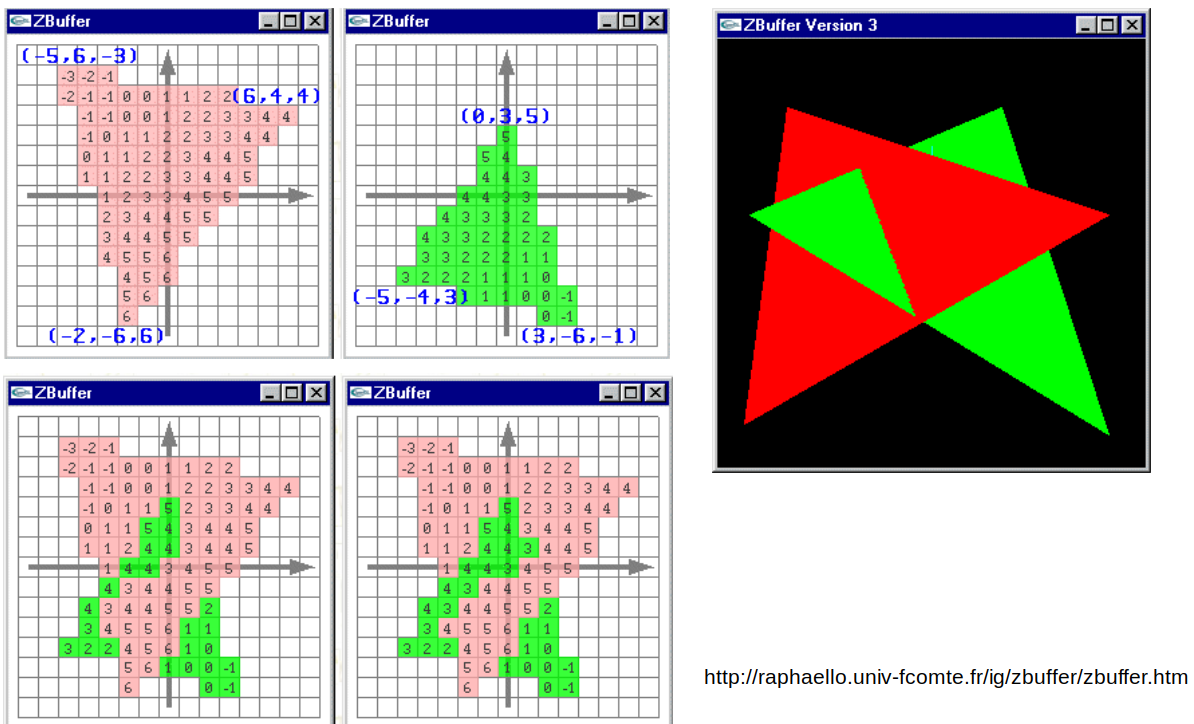
\includegraphics[width=0.75\linewidth]{img/zbuffer}}
	\caption{Иллюстрация механизма работы алгоритма буфера глубины. независимо от порядки отрисовки треугольников мы получаем нужный результат, за исключением фрагментов (пикселей), который находятся на одинаковой глубине. Эта проблема называется Z-fighting.}
	\label{fig:zbuffer}
\end{figure}

Чтобы реализовать буфер глубины, Вам необходимо создать дополнительное изображение с глубиной с разрешением буфера кадра. Вы рисуете фрагмент и обновляете значения в буфере глубины только если тест глубины проходит -- т.е. глубина текущего фрагмента меньше чем глубина, которая уже записана в z-буфер.

\paragraph{``1/z'' буфер и переспективная коррекция.} Однако есть существенный нюанс, который мы до сих пор обходили стороной. Вспомните, что при переходе от однородных координат к декартовым мы делили координаты преобразованной вершины на w. Если посмотреть как обычно формируется матрица проекции, то можно увидеть что на самом деле в случае перспективной проекции деление на w будет соответствовать делению на z координату. 

Преобразованная вершина будет состоять из следующих координат: $(x/w, y/w, z/w, 1/w)$. Если положить $w=z$, тогда $(x/z, y/z, 1, 1/z)$. То есть, после преобразования вершины в пространство NDC нам на самом деле нужны три числа: $(x/w, y/w, 1/w)$ которые условно соответствуют тройке $(x/z, y/z, 1/z)$.

Нюанс состоит в том, что поскольку в преобразовании координат из мирового пространства (или даже пространства камеры) в NDC присутствует операция деления, \textbf{нельзя просто так интерполировать значения вершинных атрибутов}, поскольку значение некоторого вершинного атрибута $A$ при этом будет будет изменяться нелинейно при движении в плоскости изображения и обратном переходе в мировое пространство. А вот значение \textbf{$A/z$ (вернее $A/w$) будет изменяться линейно!} 

Поэтому в реализацию z-буфера и интерполяции вершинных атрибутов необходим внести следующие изменения:

\begin{enumerate}
\item В z-буфере вы храните не само значение z, а значение 1/z (вернее 1/w);
\item На стадии TriangleSetUp для всех атрибутов (цвет, текстурные координаты др. если есть) вы умножаете их умножаете их значения на (1/w): \newline $tri.texCoord = texCoord*(1/w)$;
\item В каждом пикселе внутри треугольника Вы линейно интерполируете значение $(1/w)$ на основе тройки барицентрических координат;
\item Если тест глубины прошёл, Вы интерполируете при помощи тройки барицентрических координат значения атрибута поделённое на w;
\item Перед непосредственным использованием атрибута (например выборкой из текстуры) в пикселе, его значение нужно привести в исходное пространство, поделив на проинтерполированное значение обратной глубины $(1/w)$.
\end{enumerate}

\subsection{Блочный алгоритм растеризации}

Описанный алгоритм можно очевидным образом улучшить, если проверять не отдельные пиксели, а углы блоков, скажем 4x4 или 8x8 пикселей. За деталями мы рекомендуем обращаться к работе \cite{Mileff2015AcceleratedHT}. 


\begin{thebibliography}{9} 
	
\bibitem{ourtemplate} Шаблон для выполнения задания: https://github.com/FROL256/sw\_gapi\_task 

\bibitem{quadmeshes_about} Bommes, David and Lévy, Bruno and Pietroni, Nico and Puppo, Enrico and Silva, Claudio and Tarini, Marco and Zorin, Denis. Quad‐Mesh Generation and Processing: A Survey. Computer Graphics Forum (2013). 32. 10.1111/cgf.12014. 

\bibitem{quadmeshes} Подготовленные для задания меши из квадов. \newline URL = https://disk.yandex.ru/d/fX-95hx7Z8nDJA 

\bibitem{scratchpixel} Rasterization: a Practical Implementation, Scratchapixel 3.0. A free educational site that progressively introduces you to the world of computer graphics. https://www.scratchapixel.com/lessons/3d-basic-rendering/rasterization-practical-implementation/overview-rasterization-algorithm.html

\bibitem{ignatenkocoords} Алексей Игнатенко. Однородные координаты. Искать в интернете.

\bibitem{godbolt} Compiler Explorer: https://godbolt.org/

\bibitem{TnLCache} Cem Cebenoyan and Matthias Wloka. Optimizing the Graphics Pipeline. https://www.nvidia.pl/docs/IO/8228/GDC2003\_PipelinePerformance.pdf

\bibitem{Pineda} Juan Pineda. 1988. A parallel algorithm for polygon rasterization. SIGGRAPH Comput. Graph. 22, 4 (Aug. 1988), 17–20. https://doi.org/10.1145/378456.378457

\bibitem{Mileff2015AcceleratedHT} Péter Mileff, Károly Nehéz, Judit Dudra.  Accelerated Half-Space Triangle Rasterization. (2015) http://acta.uni-obuda.hu/Mileff\_Nehez\_Dudra\_63.pdf

\end{thebibliography} 

\end{document}
